\documentclass{TDP003mall}
\usepackage{graphicx}
\graphicspath{ {bilder/} }


\newcommand{\version}{Version 1.0}
\author{Gustav P Svensson, \url{gussv375@student.liu.se}\\
  Love Bäckman, \url{lovba497@student.liu.se}}
\title{Dokumentmall}
\date{2016-xx-xx}
\rhead{Daniel Persson\\
Love Backman}



\begin{document}
\projectpage

\tableofcontents
\newpage

\section{Revisionshistorik}
\begin{table}[!h]
\begin{tabularx}{\linewidth}{|l|X|l|}
\hline
Ver. & Revisionsbeskrivning & Datum \\\hline
0.1 & Ett första utkast & 16110 \\\hline
\end{tabularx}
\end{table}


\section{Spelide}
Spelet representeras i en 2D-värld, med en kamera som följer efter spelaren från sidan. Uppgiften för spelaren är att ta sig från startpunkten till målet så snabbt som möjligt. Påvägen till målet kan spelaren stöta på hinder, till exempel fåglar eller kvicksand, som påverkar spelarens hastighet.
\\\\
Den bästa tiden för varje barna kommer sparas så att spelaren har ett mål att slå.
\\\\
I mån av tid kommer även online multiplayer implementeras vilket medför ytterligare ett tävlingsmoment.
\\\\
Då det är ett racingspel med ambition att implementera online multiplayer existerar det inte några fiender som kan döda en spelare, eftersom det försämrar tävlingsmöjligheterna då tillfälligheter kan få katastrofala konsekvenser för racet.


\section{Målgrupp}
Spelets målgrupp är personer i alla åldrar som gillar utmanande platformsracingspel.

\section{Spelupplevelse}
Det som gör spelet underhållande att spela är att det är utmanande och strävan att alltid bli bättre, att alltid
få bättre tid. Att få till en ``perfect run'' då man klarar barnan på den bästa möjliga tiden är något som spelare alltid kan sträva efter då det är otroligt svårt att få klara av.\newline
Man kan även välja att spela olika barnor vilket inte gör spelet enformigt då det finns hinder på olika ställen beroende på vilken barna man kör.

\newpage

\section{Spelmekanik}
\subsection{In-game}
Spelaren kan röra sig i sidled samt hoppa.
Kameran kommer flytta sig så den följer med spelaren hela tiden, det vill säga, spelaren kommer alltid vara centrerad på skärmen.
\\\\
NPC:erna kommer röra sig enligt en förbestämmd algoritm för varje bana. Följande NPC:er kommer finnas i spelet:
\\\\
\begin{tabular}{|l|l|}
\hline
\textbf{NPC} & \textbf{Effekt vid kollision} \\\hline
Slowing bird & Spelarens hastighet minskar i 5 sekunder. \\\hline
Boost bird & Spelarens hastighet ökar i 5 sekunder. \\\hline
Net from boost bird & Spelaren kan inte röra sig i 2 sekunder. \\\hline
Kvicksand & Spelarens hastighet minskar fram tills man nuddar vanlig mark \\\hline
Boost block & Spelarens hastighet ökar tills man nuddar vanlig mark. \\\hline
\end{tabular}
\\\\
\\
I mån av tid kommer vi implementera ett system som kommer öka spelarens hastighet beroende på hur många gånger som spelaren har hoppat med sidorörelse utan att kollidera med andra objekt än marken.
\\\\
\begin{tabular}{|c|c|}
\hline
\textbf{Knapptryck} & \textbf{Händelse} \\\hline
W eller $\uparrow$ & Spelaren hoppar \\\hline
A eller $\leftarrow$ & Spelaren går åt vänster \\\hline
D eller $\rightarrow$ & Spelaren går åt höger \\\hline
ESC & Öppna spelmenyn \\\hline
\end{tabular}

\subsection{Meny}
I startmenyn kan man välja vilken bana man vill spela. \\
I mån av tid ska det även gå att göra en online-session så man kan spela med sina vänner.

\section{Regler}

\subsection{Allmänt}
Banan är slut när spelaren har nått målet. \\
I mån av tid så ska banan vara slut när alla spelare har kommit i mål eller efter ett fördefinierat antal sekunder från dess att den första spelaren har kommit i mål.

\subsection{Spelarregler}
Spelaren ska bara kunna röra sig i sidled samt hoppa uppåt. Spelaren ska inte kunna gå igenom block, spelet ska alltså hålla koll på spelarens position samt blockens position. Vid kollision mellan en spelare och ett block ska spelaren inte längre kunna röra sig åt det hållet som blocket är placerat. \newline
I mån av tid ska spelaren även kunna hoppa på väggar, förutsatt att spelaren igen inom en utsatt tid.
I mån av tid ska spelaren även kunna få högre hastighet om den hoppar flera gånger i rad, förutsatt att spelaren hoppar med en sidorörelse utan att kollidera med något annat solidt block förrutom marken. \newline
\\
Spelaren startar på en fördefinierad position beroende på vilken bana som körss.-

\\\\
Om en spelare kolliderar med en slow bird så kommer spelarens hastighet minska med ett fördefinierat värde. \\
Om en spelare kolliderar med en Boost bird så kommer spelarens hastighet öka med ett fördefinierat värde. \\
Om en spelare kolliderar med ett NFBB ( Net from boost bird ) så kommer spelaren att tappa förmågan att röra sig i ett fördefinierat antal sekunder.
\\\\
Om en spelare befinner sig i ett air block så ska spelaren börja röra sig i air blockets vindriktning och dens hastighet. \\
Om en spelare befinner sig på ett quicksand block så ska spelarens hastighet sänkas med ett fördefinierat värde. \\
Om en spelare befinner sig på ett goalblock så har spelaren kommit i mål och kan därmed inte röra sig längre.



\subsection{NPC:er}
\subsubsection{Slow bird}
Slow birds är inte ett solidt block. \\
Slow birds spawnar efter en utsatt tid, beroende på vilken bana spelaren spelar. Slow bird flyger, och kan endast flyga i sidled. När den kolliderar med ett block så kommer den byta riktning i sidled. \\
I mån av tid så ska slow birden flyga efter en cos- eller sinuskurva istället för att flyga i en rak linje.

\subsubsection{Boost bird}
Boost birds är inte ett solidt block. \\
Boost birds spawnar efter en utsatt tid, beroende på vilken bana spelaren spelar. Boost bird flyger, och den kan endast flyga i sidled. När den kolliderar med ett block så kommer den byta riktning i sidled. \\
Inom ett utsatt interval så ska boost bird:en släppa ett nät som heter ``Net from boost bird''.

\subsubsection{Net from boost bird}
Net from boost bird är inte ett solidt block. \\
``Net from boost bird'', förkortas NFBB, spawnas av Boost bird i ett utsatt interval. NFBB faller med en fast hastighet enligt en lodrät linje, utifrån den punkten den släpptes från boost bird:en. När den kolliderar med ett block så ligger den där i ett utsatt antal sekunder innan den despawnar.

\subsection{Block}

\subsection{Icke solida block}
Icke solida block är en typ av block som spelare och NPC:er kan passera igenom.

\subsubsection{Air block}
I mån av tid så ska air block implementeras. Air block är statiska, de ska alltså inte kunna röra sig. \\
Ett air block simulerar vind, den har en vindriktning och en fördefinierad vindhastighet.

\subsection{Solida block}
Solida block är block som spelare och NPC:er inte kan passera igenom.

\subsubsection{Goalblock}
Ett goalblock är ett solidt block som r statiskt, den kan alltså inte röra på sig. \\


\subsubsection{Quicksand}
Quicksand är ett solidt block som är statisk, den kan alltså inte röra på sig. \\
I mån av tid så bör quicksand kunna röra på sig om det ligger på ett block som rör sig.

\subsubsection{Terrain}
Terrain är ett solidt block som kan röra sig i sidled samt i höjdled. Dessa block finns i olika texturer.

\section{Visualisering}
\subsection{Meny}
När spelaren startar spelet så kommer den mötas utav huvudmenyn. Här får spelaren två simpla val, ``select level'' och ``exit''. \\
Om spelaren trycker på ``select level'' så kommer levelmenyn öppnas. Levelmenyn består av bilder samt en tillbaka knapp. Trycker spelaren på tillbacka knappen så kommer levelmenyn stängas och huvudmenyn öppnas igen. \\
På varje bild så kommer det stå namnet på banan, om spelaren trycker på en bild så kommer den banan att startas.

\begin{figure}[h]
  \centering
  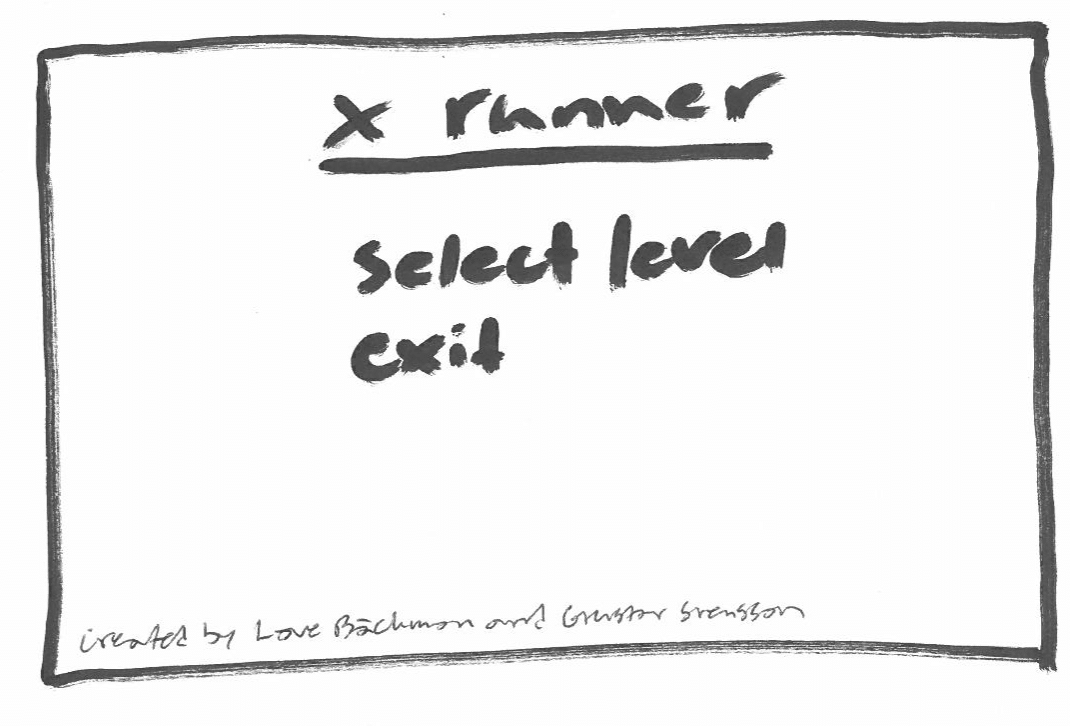
\includegraphics[scale=0.15]{startmeny}
  \caption{Startmenyn}
  \label{Startmenyn}
\end{figure}

\begin{figure}[h]
  \centering
  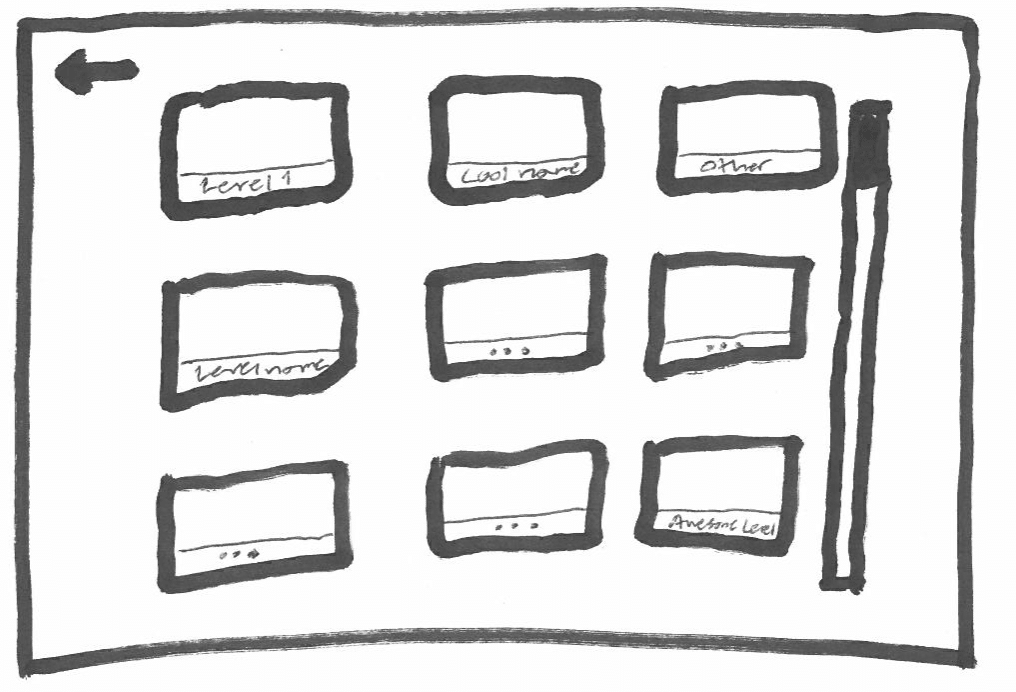
\includegraphics[scale=0.15]{levelmeny}
  \caption{Levelmenyn}
  \label{Levelmenyn}
\end{figure}

\newpage
\subsection{Spelplan}
När spelaren har valt en bana så kommer den banan att laddas upp. Spelplanen kommer se annorlunda ut beroende på bilken bana spelaren valde. \\
Spelplanen består av NPC:er, block och spelaren själv. \\
På spelplanen så kan spelaren och NPC:er röra sig.

\begin{figure}[h]
  \centering
  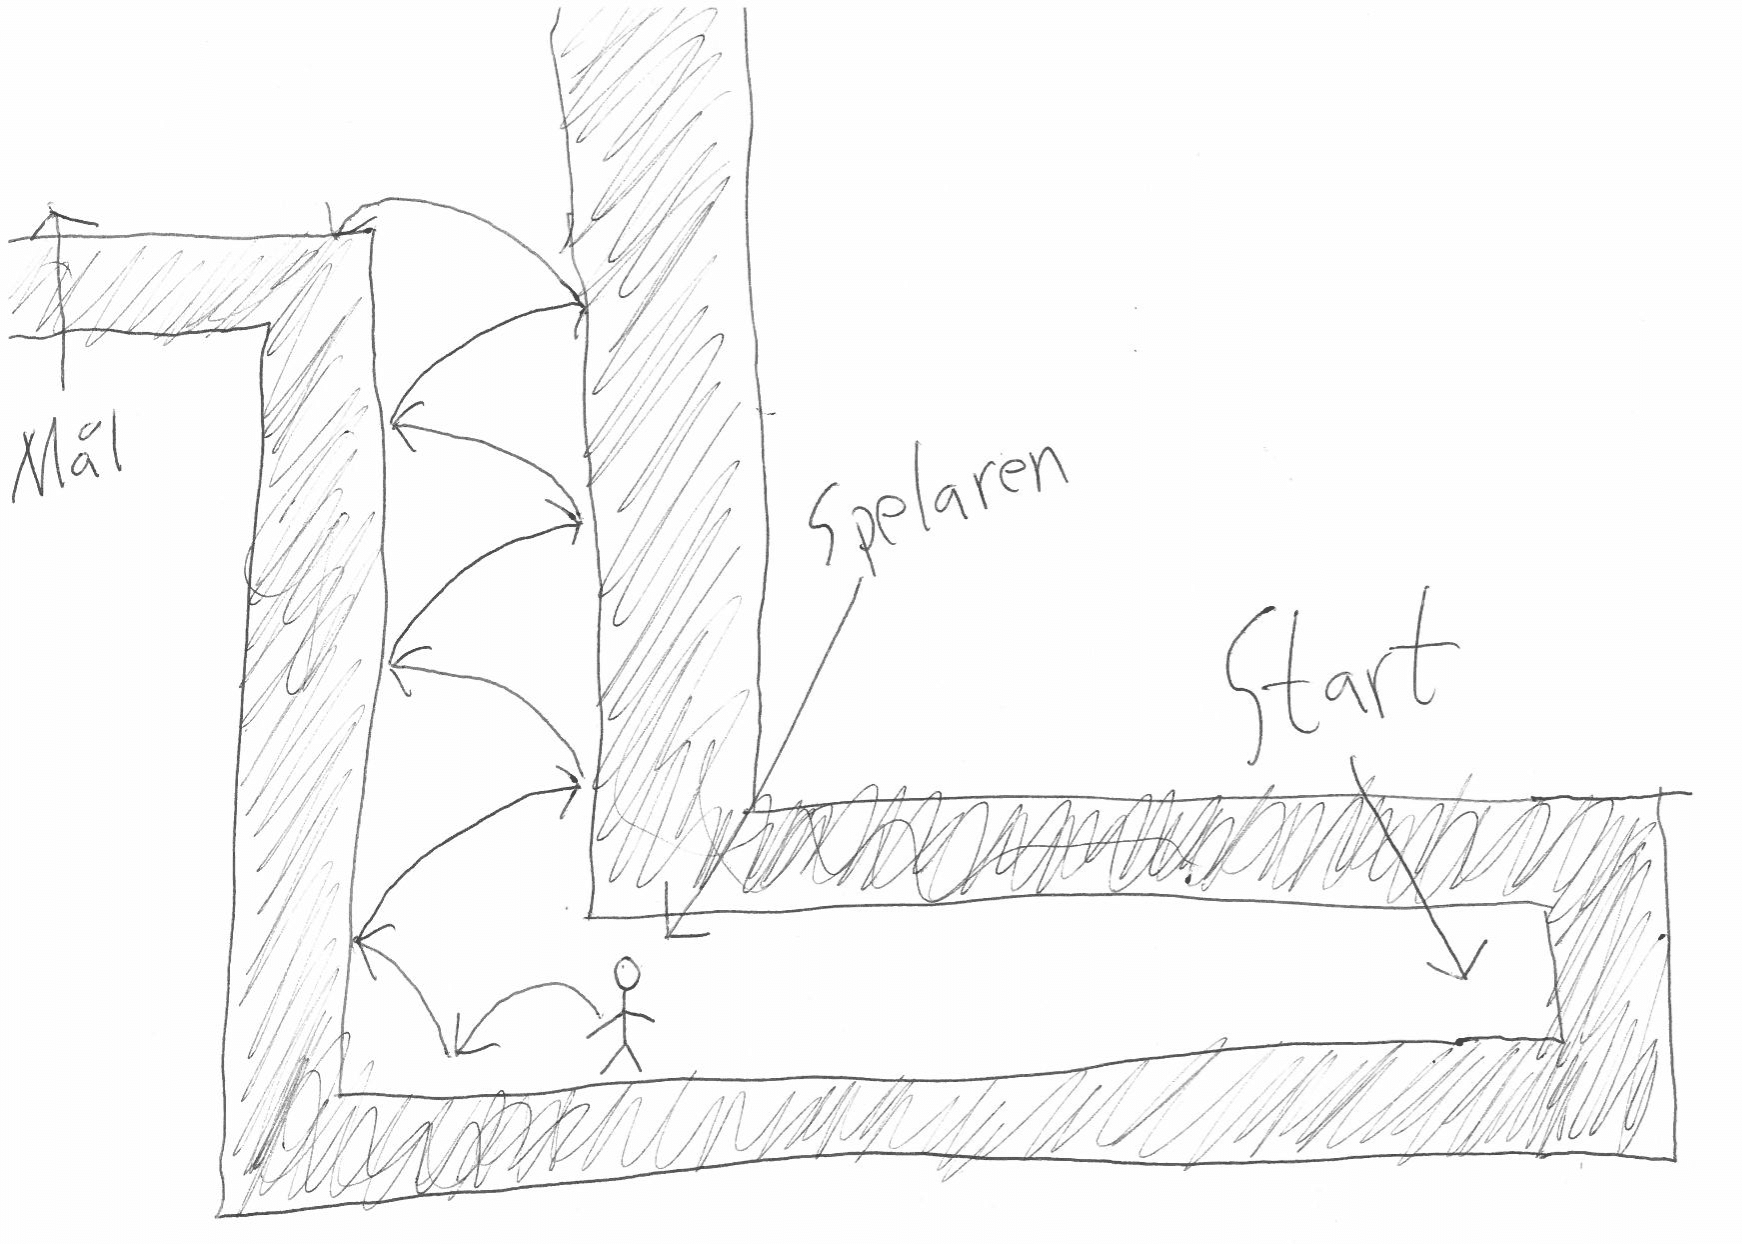
\includegraphics[scale=0.10]{success}
  \caption{Skiss på en lyckad ``wall jump''}
  \label{Skiss på en lyckad ``wall jump''}
\end{figure}

\begin{figure}[h]
  \centering
  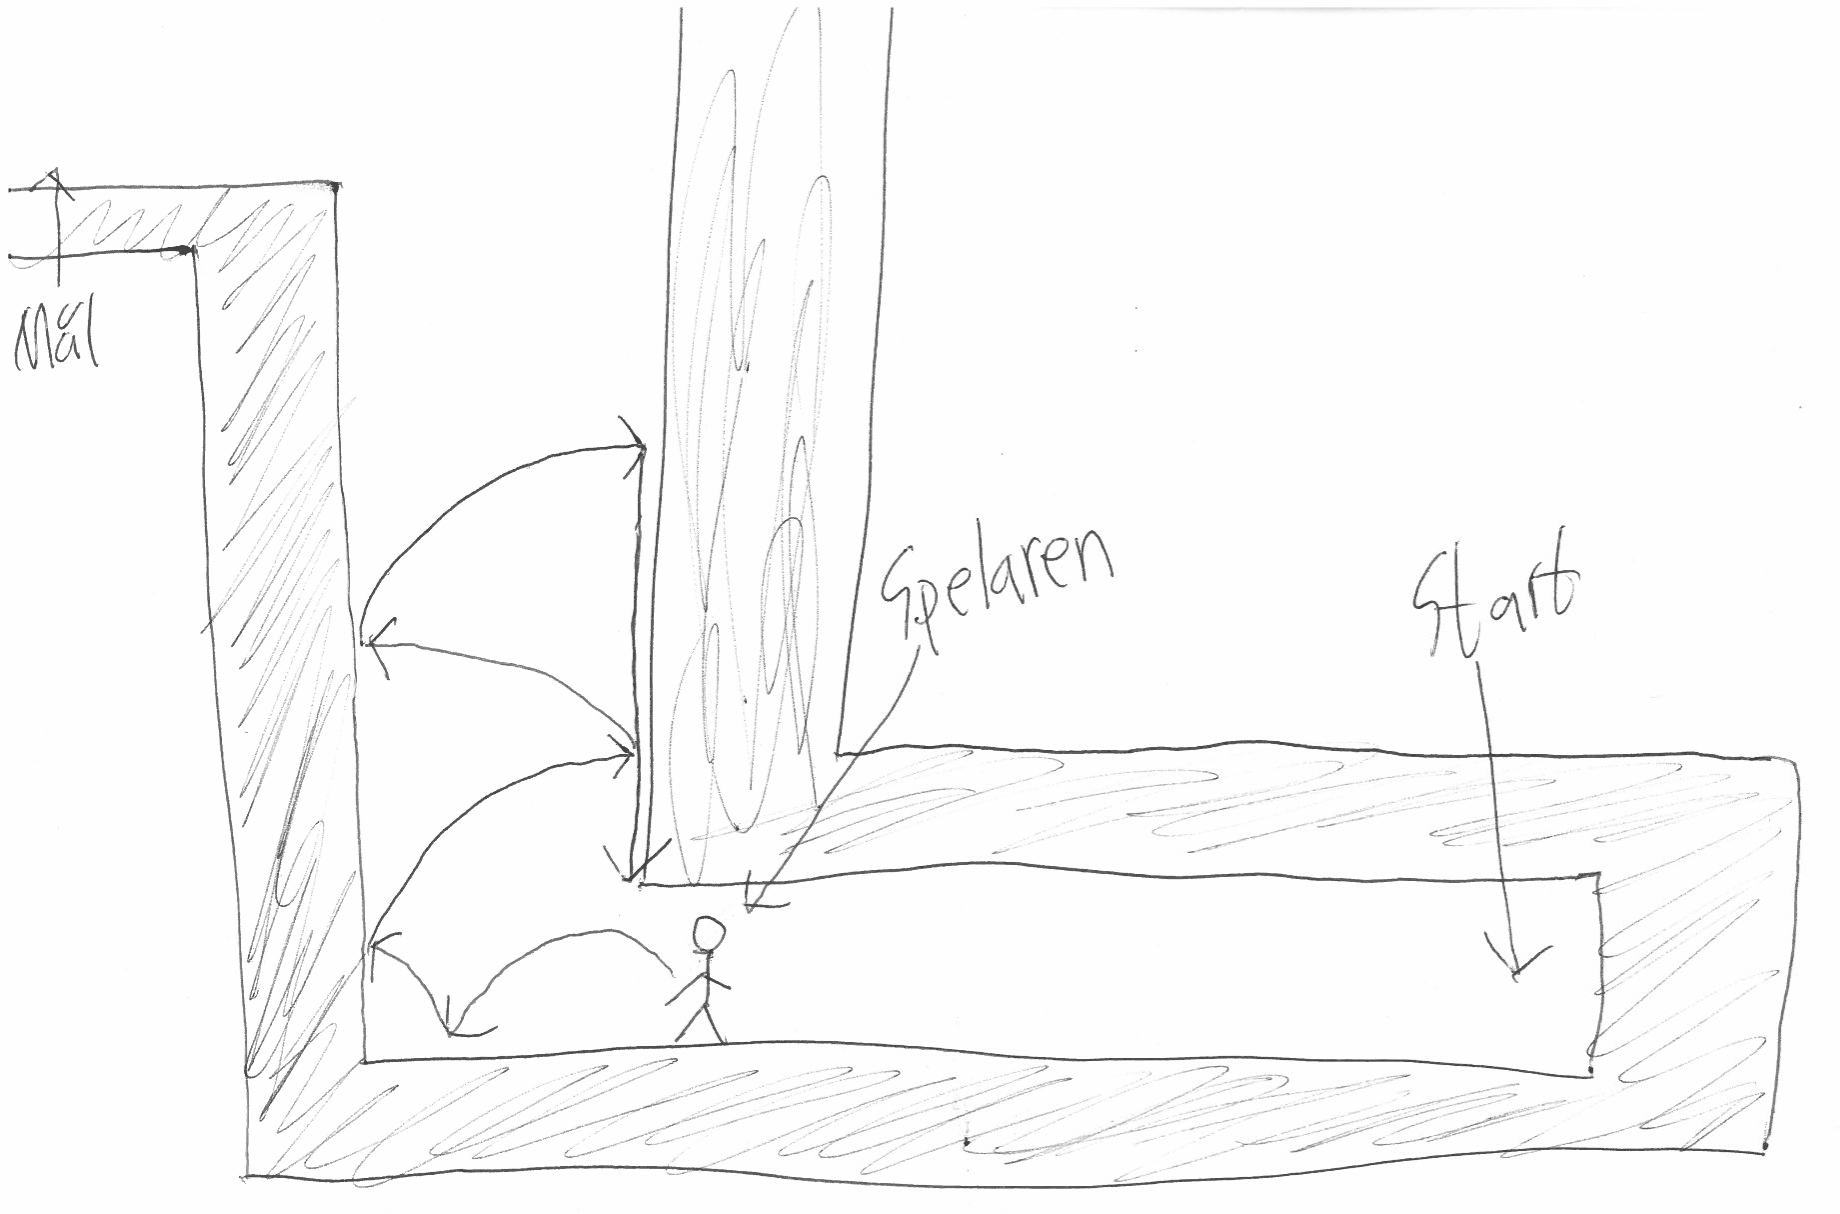
\includegraphics[scale=0.10]{fail}
  \caption{Skiss på en misslyckad ``wall jump''}
  \label{Skiss på en misslyckad ``wall jump''}
\end{figure}

\newpage

\section{Kravformulering}
\subsection{Ska-krav}
\begin{itemize}
\item Spelaren ska kunna flytta sig i sidled och hoppa med tangentbordet.
\item Den valda banan ska kunna målas ut.
\item NPC:er ska kunna röra sig.
\item Det ska kunna finnas flera NPC:er på banan.
\item Inga objekt ( Allting som finns på spelplanen ) ska kunna passera igenom solida block.
\item När spelaren nuddar ett goalblock så ska spelaren ha klarat banan.
\item Spelaren ska alltid vara centrerad på skärmen.
\end{itemize}

\subsection{Bör-krav}
\begin{itemize}
\item Spelet ska spara den bästa tid på varje bana.
\item Man ska kunna spela online multiplayer.
\item Spelarens hastighet ska öka när spelaren hoppar flera gånger i rad utan att kollidera med ett solidt block.
\item Spelaren ska kunna göra ``wall jumps'' genom att hoppa inom en fördefinierad tidsram efter att spelaren har kolliderat med ett solidts blocks vägg.
\item Den bästa för den nuvarande banan ska synas på skärmen.
\item När spelaren nuddar en NPC utförs den ovan definierade händelsen.
\item När spelaren eller NPC:er nuddar ett block så utförs den ovan definierade händelsen.
\item Spelaren ska påverkas av gravitation.
\end{itemize}

\section{Kravuppfyllelse}
\textit{Spelet ska simulera en värld som innehåller olika typer av objekt. Objekten ska ha olika beteenden och röra
sig i världen och agera på olika sätt när de möter andra objekt.}
\begin{itemize}
\item Varje bana har flera olika typer av block och NPC:er som alla har olika beteenden och egenskaper samt interagerar med varandra och spelaren.
\end{itemize}


\noindent\textit{Det måste finnas minst tre olika typer av objekt och det ska finnas flera instanser av minst två av dessa.
T.ex ett spelarobjekt och många instanser av två olika slags fiendeobjekt.}
\begin{itemize}
\item Spelet har flera olika typer av objekt, olika blockobjekt, två olika NPC:er samt spelaren. Det kommer finnas flera olika instancer av dessa.
\end{itemize}

\noindent\textit{Ett beteende som måste finnas med är att figurerna ska röra sig över skärmen. Rörelsen kan följa ett
mönster och/eller vara slumpmässig. Minst ett objekt, utöver spelaren ska ha någon typ av rörelse.}
\begin{itemize}
\item Spelaren ska kunna röra sig i höjdled samt sidled och påverkas av gravitation. NPC:er kommer även kunna röra sig i sidled, eventuellt enligt en sin-/cosinus kurva.
\end{itemize}

\noindent\textit{En figur ska styras av spelaren, antingen med tangentbordet eller med musen. Du kan även göra ett spel där
man spelar två stycken genom att dela på tangentbordet (varje spelare använder olika tangenter). Då styr
man var sin figur.}
\begin{itemize}
\item Spelaren styr sin karaktär genom att använda tangentbordet.
\end{itemize}

\noindent\textit{Grafiken ska vara tvådimensionell.}
\begin{itemize}
\item Ja, vi använder 2D-grafik med hjälp av SFML.
\end{itemize}

\noindent\textit{Världen (spelplanen) kan antas vara lika stor som fönstret (du kan göra en större spelplan med scrollning,
men det blir lite krångligare).}
\begin{itemize}
\item Spelplanen kommer använda scrolling så ja, detta uppfylls.
\end{itemize}

\textit{Det ska finnas kollisionshantering, det vill säga, det ska hända olika saker när objekten möter varandra, 
de ska påverka varandra på något sätt. T.ex kan ett av objekten tas bort, eller så kan objekten förvandlas på
något sätt, eller så kan ett nytt objekt skapas.}
\begin{itemize}
\item Ja, detta uppfylls. När spelaren kolliderar med solida block eller med NPC:er samt när NPC:er kolliderar med solida block.
\end{itemize}

\noindent\textit{Spelet måste upplevas som ett sammanhängande spel som går att spela!}
\begin{itemize}
\item Ja det kommer det att göra.
\end{itemize}

\end{document}
